\documentclass[../../main.tex]{subfiles}
\begin{document}

\section{Лекция 3. 7 ноября 2019 г.}
\vspace{10pt}

{\large База и предбаза топологии. Примеры. Критерий существования топологии с данной (пред)базой. Пример: топология поточечной сходимости. Сходимость последовательностей в топологическом пространстве. База и предбаза в точке. Описание сходимости в метрическом пространстве. Замыкание множества в топологическом пространстве. Свойства операции замыкания. Предельные и изолированные точки.}

\vspace{10pt}




\begin{minipage}{0.75\linewidth}
\textbf{Лемма.} $X$ — множество, $\beta \subset 2^X$. Следующие свойства множества $A \subset X$ эквивалентны:

(1) $\ex \gamma \subset \beta \colon A = \cup \gamma$  

(2) $\fo x \in A \ex B \in \beta \colon x \in B \subset A$

\textbf{Доказательство} (1) $\Ra$ (2)

Пусть $A = \cup \gamma, \gamma \subset \beta, x \in A \Ra \ex B \in \gamma \colon x \in B \Ra B \text{ удовл. (2)}$

(2) $\Ra$ (1) $\fo x \in A \ex B \in \beta \colon x \in B_x \subset A \Ra \gamma = \left\{ B_x \colon x \in A \right\} \text{ удовл. (1)}$
\end{minipage}
\begin{minipage}{0.25\linewidth}

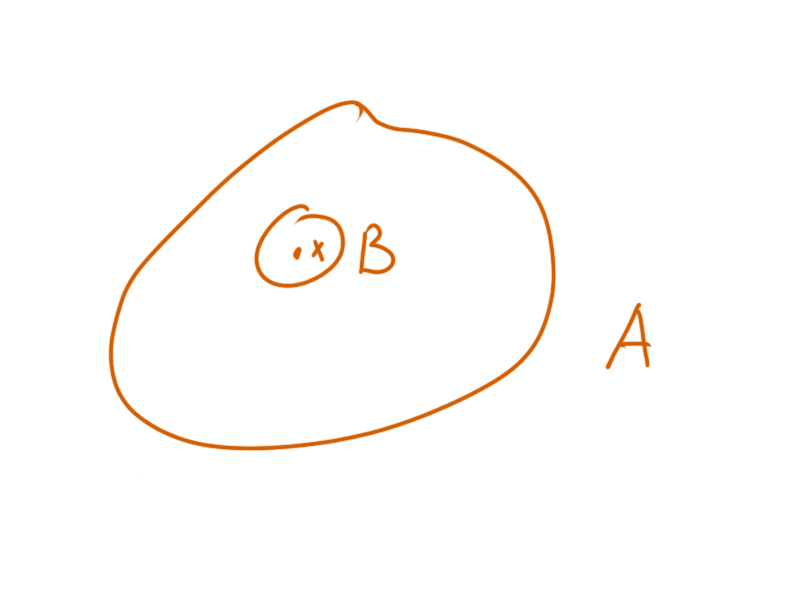
\includegraphics[width = 4cm]{pictures/1.jpg}

$\gamma \subset 2^X$

Обозначение: $\bigcup_{C \in \gamma} C = \cup \gamma$
\end{minipage}

\defn $\left(X, \tau \right)$ — топологическое пространство

(1) $\beta \subset \tau $ — база топологии $\tau$ (или база $\left(X, \tau \right)$) $\lra$ кажд. $U \in \tau$ является объединением некоторого подсемейства в $\beta \xLeftrightarrow[\text{лемма}]{}{} \fo U \in \tau \fo x \in U \ex B \in \beta \colon x \in B \subset U $

(2) $\sigma \subset \tau$ — предбаза $\tau$ (предбаза $\left(X, \tau \right)$) $\lra$ семейство $\left\{ U_1 \cap \ldots \cap U_n \colon U_i \in \sigma, \;\; n \in \N \right\}$

\textbf{Пример.} $\left( X, \ro \right)$ — метрическое пространство $\Lra \left\{ B_r(x) \colon x \in X, r > 0 \right\}$ — база $\tau_{\ro}$

\textbf{Пример:} $X = \R \quad \sigma = \left\{(—\infty;\: b); (a, +\infty) \colon a,b \in \R \right\}$ — предбаза $\R$, но не база.

\begin{minipage}{0.8\linewidth}
\textbf{Предложение} $X$ — множество, $\;\; \beta, \sigma \subset 2^X$

(1) На $X \; \ex$ топология с базой $\beta \lra 
\begin{cases} 
(a) \cup \beta = X \\
(b) \fo B_1, B_2 \in \beta\; \fo x \in B_1 \cap B_2 \quad \ex B_3 \in \beta \colon x \in B_3 \subset B_1 \cap B_2
\end{cases}$

(2) На $X \; \ex$ топология с предбазой $\sigma \lra \cup \sigma = X$
\end{minipage}
\begin{minipage}{0.2\linewidth}
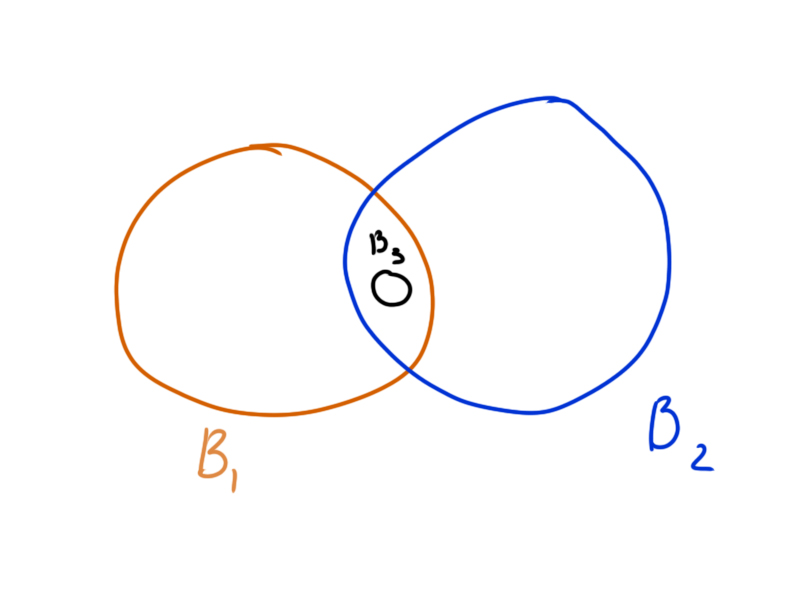
\includegraphics[width=4cm]{pictures/2.jpg}
\end{minipage}

\textit{Доказательство:} (1) ($\Ra$) следует из открытости $X$  $B_1 \cap B_2$

Обозначим $\tau = \left\{ \cup \gamma \colon \gamma \subset B  \right\}$. Покажем $\tau$ — топология на $X$

$\varnothing = \cup \varnothing \in \tau; \; X = \cup \beta \in \tau; $ объединение множеств из $\tau$ принадлежит $\tau$

Пусть $U_1, U_2 \in \tau$. Хотим: $ U_1 \cap U_2 \in \tau$

Пусть $x \in U_1 \cap U_2 \Lra \ex B_1, B_2 \in \beta \colon x \in B_k \subset U_k \;\; (k = 1, 2) \Ra x \in B_1 \cap B_2 \xRightarrow[\text{(b)}]{} \ex B_3 \in \beta \colon x \in B_3 \subset B_1 \cap B_2 \subset U_1 \cap U_2 \Lra_{\text{л}} U_1 \cap U_2 \in \tau \Ra \tau $ — топология на $X$, и $\beta$ — её база.

(2) ($\Ra$) из открытости $X$

($\Leftarrow$) Семейство $\left\{ U_1 \cap \ldots \cap U_n \colon U_i \in \sigma,\: n \in \N \right\}$ удовл. (a), (b) $\Ra$ оно — база топологии, а $\sigma$ — её предбаза. $\square$

\vspace{10pt}
\begin{minipage}{0.7\linewidth}
\textbf{Пример.} (топология поточечной сходимости)

Пусть $\K = \R$ или $\mathbb{C}\;\;$, $S \subset \K^X \quad$ (где $X$ — любое множество)

$\fo x \in X,$ для каждого интервала (для $\K = \mathbb{C}$ — открытый круг) $I \subset \R$ обозначим $G(x, I) = \left\{ f \in S \colon f(x) \in I \right\}$

Семейство $\left\{ G(x, I) \colon x \in X, I \subset \R \text{ — интервал (для } \K = \mathbb{C} \text{— открытый круг)} \right\}$ является предбазой некоторой топологии на $S$. Она называется \textit{топологией поточечной сходимости} на $S$
\end{minipage}
\begin{minipage}{0.3\linewidth}
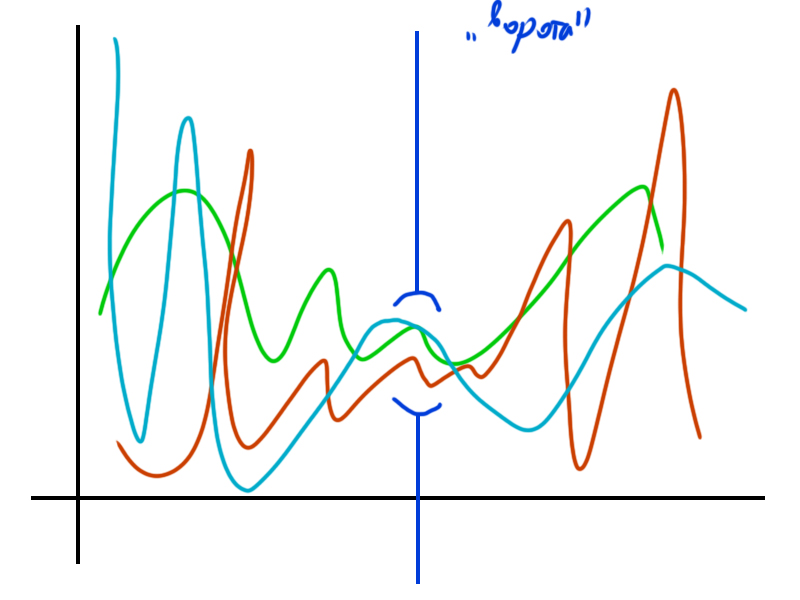
\includegraphics[width=5cm]{pictures/3.jpg}
\end{minipage}

\subsection{Сходимость последовательностей в топологическом пространстве}

$X$ — топологическое пространство, $x \in X,\;\; (x_n)$ — последовательность в $X$.

\defn $(x_n)$ \textit{сходится} к $x$ ($x$ является \textit{пределом} $(x_n)$) $\lra \fo \text{ окрестности } U \ni x \; \ex N \in \N \;\; \fo n \geq N \; x_n \in U$

\textit{Обозначение} $x_n \rightarrow x \;\; (n \rightarrow \infty)$, или $x = \lim_{n \to \infty} x_n$

\defn (1) Семейство $\beta_x$ окрестностей точки $x \in X$ — \textit{база окрестностей} $x$ (\textit{база} в $x$) $\lra$ для любой окрестности $U \ni x \;\; \ex V \in \beta_x \subset U$

(2) Семейство $\sigma_x$ окрестностей точки $x \in X$ — \textit{предбаза окрестностей} $x$ (\textit{предбаза} в $x$) $\lra \left\{ U_1 \cap \ldots \cap U_n \colon U_i \in \sigma_x,\; n \in \N \right\}$ — база в $x$.

\begin{minipage}{0.5\linewidth}
\textbf{Пример.} $\left(X, \ro \right)$ — метрическое пространство.

$\left\{ B_r(x) \colon r > 0 \right\}$ — база в $x$

$\left\{B_{\frac 1 n}(x) \colon n \in \N \right\}$ — тоже

\end{minipage}
\begin{minipage}{0.2\linewidth}
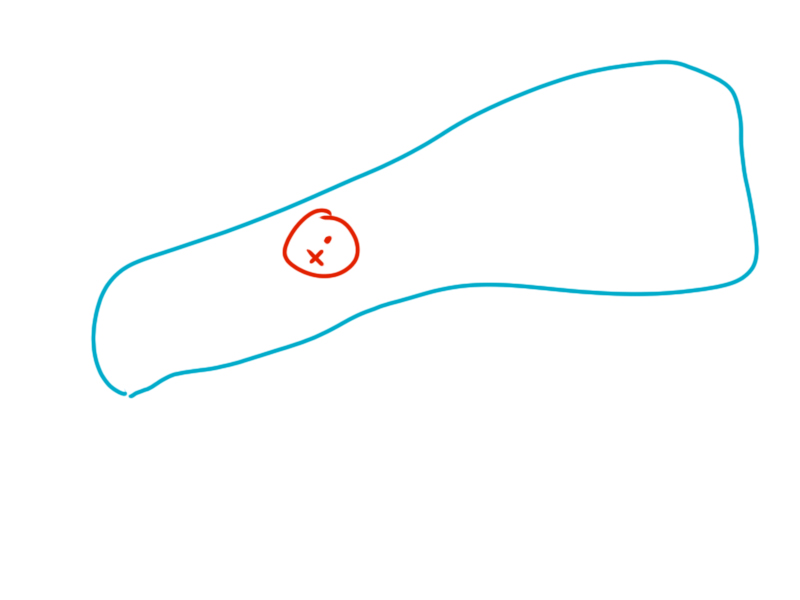
\includegraphics[width=4cm]{pictures/4.jpg}
\end{minipage}

\textbf{Предложение} $X$ — топологическое пространство, $x \in X$, $\sigma_x$ — предбаза в $x$, $(x_n)$ — последовательность в $X$.
$$x_n \to x (n \to \infty) \lra \fo V \in \sigma_x \; \ex\; N \in \N \; \fo n \geq \N \; x_n \in V$$

\textit{Доказательство:} ($\Leftarrow$) Пусть $U$ — окрестность $x$ $\Ra \ex \; V_1, \ldots, V_p \in \sigma_x \colon V_1 \cap \ldots \cap V_p \subset U$

$\ex N_1, \ldots, N_p \colon \fo n \geq N_i \;\; x_n \in V_i \quad (i = 1, \ldots, p)$

Обозначим $N = \max_{1 \leq i \leq n} N_i \Ra \fo n \geq N \quad x_n \in V_1 \cap \ldots \cap V_p \subset U \;\; \square$

\textit{Следствие} $\left(X, \ro \right)$ — метрическое пространство, $x \in X, (x_n)$ — последовательность в $X$. Следующие утверждения эквивалентны:

(1) $x_n \to x$

(2) $\fo$ открытого шара $U$ с центром в $x \; \ex\; N \in \N\;\; \fo n \geq N \;\; x_n \in U$

(3) $\fo\; \eps > 0 \; \ex N \in \N \;\; \fo n \geq N \;\; \ro(x_n, x) < \eps$

(4) $\ro(x_n, x) \to 0$

\textit{Предложение.} $X$ — хаусдорфово топологическое пространство, $(x_n)$ — последовательность в $X,\quad x_n \to x \in X, x_n \to y \in X \Ra x = y$

\textit{Доказательство:} пусть $x \neq y \Ra \ex$ окрестности $U \ni x, V \ni y, U \cap V = \varnothing$

$\left.
\begin{gathered}
\ex N_1 \colon \; \fo n \geq N_1,\; x_n \in U  \\
\ex N_2 \colon \; \fo n \geq N_2 \; x_n \in V 
\end{gathered}
\right\}  
\Ra x_n \in U \cap V\;\; \fo n \geq max\left\{N_1, N_2 \right\}  $ — противоречие. $\square$

\textbf{Пример.} $X$ — антидискретное топологическое пространство

Каждая последовательность в $X$ сходится к каждой точке $x \in X$

\textbf{Пример.} $X$ — дискретное топологическое пространство

$x_n \to x \lra \ex N \in \N \;\; \fo n \geq N \;\; x_n = x$

Действительно: ($\Ra$) $\left\{x \right\}$ — окрестность $x$. Далее см. определение сходимости.

\textbf{Пример-упражнение.}

$\K = \R$ или $\mathbb{C}$, $X$ — множество, $S \subset \K^X$

Пусть $f_n \to f$ в $S$ с топологией поточечной сходимости $\lra \fo x \in X \;\; f_n(x) \to f(x)$

\subsection{Замыкание, внутренность, граница ...}

$X$ — топологическое пространство, $A \subset X$

\defn \textit{Замыкание} $A$ — множество $\overline{A} = \bigcap \left\{F \subset X\; \colon\; F \text{ замк}, F \supset A \right\}$

\textit{Наблюдение.} $\overline{A}$ — наименьшее замкнутое множество, содержащее $A$. (В частности, если $A$ замкнуто, то $A = \overline{A}$).

\textit{Предложение.} 

(1) $A \subset B \subset X \Ra \overline{A} \subset \overline{B}$

(2) $\overline{\overline{A}} = \overline{A}$

(3) $\overline{A \cup B} = \overline{A} \cup \overline{B}$

\textit{Доказательство:} (1) из опр. (2) из наблюдения

(3) $A \subset A \cup B \Ra^{(1)} \overline{A} \subset \overline{A \cup B}$. Аналогично, $\overline{B} \cup \overline{A \subset B} \Ra \overline{A} \cup \overline{B} \subset \overline{A \cup B}$

$A \cup B \subset \overline{A} \cup \overline{B} \Ra^{(1)} \overline{A \cup B} \subset \overline{\overline{A} \cup \overline{B}} = \overline{A} \cup \overline{B}$, т.к. $\overline{A} \cup \overline{B}$ замкнуто. $\square$.


\textit{Предложение.} $x \in \overline{A} \lra \fo $ окрестности $U \ni x \quad U \cap A \neq \varnothing$.

\textit{Доказательство:} 

$x \notin \overline{A} \lra \ex $ замкн. $F \subset X \colon F \supset A, x \notin F \xLeftrightarrow[U = x \backslash F]{}{} \ex $ откр $U \subset X \colon \; U \cap A = \varnothing,$ и $x \in U \lra \ex\;$ окр $U \ni x,\;\; U\cap A = \varnothing \;\; \square$

\defn $X$ — топологическое пространство, $A \subset X$

$x \in X$ — \textit{предельная точка} $A \Longleftrightarrow x \in \overline{A \backslash \{ x\}}, \xLeftrightarrow[\text{предл.}]{}{}$ в каждой окрестности $x$ есть точки из $A$, отличные от $x$.

$A' = \left\{x \in X \colon\; x \text{ — предельная точка } A \right\}$ — \textit{производное множество} множества $A$

Из предл. $\overline{A} = A \cup A'$. В частности: $A$ замкнуто $\lra \; A' \subset A$

\defn $x \in A$ — \textit{изолированная точка} $A\; \lra x \in A \backslash A' \; \lra \; \ex$ окрестность $U \ni x \; \colon\; U \cap A = \{ x \}$

$\overline{A} = A'$ {изолированные точки $A$}.

\end{document}